\documentclass[12pt]{article}
\usepackage{amsmath}
\usepackage{physics}
\usepackage{graphicx}
\usepackage{enumitem}

\usepackage{listings} % Required for insertion of code
\usepackage{xcolor} % Required for custom colors

% Define custom colors
\definecolor{codegreen}{rgb}{0,0.6,0}
\definecolor{codegray}{rgb}{0.5,0.5,0.5}
\definecolor{codepurple}{rgb}{0.58,0,0.82}
\definecolor{backcolour}{rgb}{0.95,0.95,0.92}

% Setup the style for code listings
\lstdefinestyle{mystyle}{
    backgroundcolor=\color{backcolour},   
    commentstyle=\color{codegreen},
    keywordstyle=\color{magenta},
    numberstyle=\tiny\color{codegray},
    stringstyle=\color{codepurple},
    basicstyle=\ttfamily\footnotesize,
    breakatwhitespace=false,         
    breaklines=true,                 
    captionpos=b,                    
    keepspaces=true,                 
    numbers=left,                    
    numbersep=5pt,                  
    showspaces=false,                
    showstringspaces=false,
    showtabs=false,                  
    tabsize=2
}

% Activate the style
\lstset{style=mystyle}


\author{Patryk Kozlowski}
\title{Homework 1}
\date{\today}
\begin{document}
\maketitle
\section{Problem 1}
Ashcroft and Mermin, Chapter 2, Problem 1
\subsection{Part a}
What is the relation between $n$ and $k_F$ in two dimensions?
\subsubsection{Solution}
By definition, the number of particles is an integral over the density of states that are singly occupied, i.e., up to the Fermi wave vector. In two dimensions, the density of states is given by
\begin{equation}
    N = \int_{0}^{k_F} \frac{d^2k}{(2\pi)^2}
\end{equation}
Expanding in polar coordinates, we have
\begin{equation}
    N = \int_{0}^{k_F} \int_{0}^{2\pi } \frac{d\theta}{(2\pi)^2} k \, dk = \frac{1}{2\pi}\int_{0}^{k_F} k \, dk = \frac{k_F^2}{2\pi}
\end{equation}
The particle density is defined as the number of particles per unit area. Since we have a unit area, then
\begin{equation}
    n = \frac{N}{A} = \frac{k_F^2}{2\pi}
\end{equation}
\subsection{Part b}
What is the relation between $k_F$ and $r_s$ in two dimensions?
\subsubsection{Solution}
The Wigner-Seitz radius is defined as the area per particle in real space. So in two dimensions, this is simply the area of a circle with radius $r_s$: $A = \pi r_s^2$. The particle density is defined as the number of particles per unit area. Since we have defined the area above, we can write
\begin{equation}
    n = \frac{N}{A} = \frac{N}{\pi r_s^2}  
\end{equation}
But then we also found that the particle density can be expressed in terms of the Fermi wave vector, so we have a relationship between the Wigner-Seitz radius and the Fermi wave vector
\begin{equation}
    n = \frac{k_F^2}{2\pi} = \frac{N}{\pi r_s^2} \implies k_F = \frac{\sqrt{2N}}{r_s}
\end{equation}
\subsection{Part c}
Prove that in two dimensions the free electron density of levels \( g(E) \) is a constant independent of \( \epsilon \) for \( \epsilon > 0 \), and 0 for \( \epsilon < 0 \). What is the constant?
\subsubsection{Solution}
A free electron only has the energy contribution from its kinetic part
\begin{equation}
    \epsilon = \frac{\hbar^2 k^2}{2m} \implies k = \sqrt{\frac{2m\epsilon}{\hbar^2}}
\end{equation}
Now the number of single particle states up to this momentum \( k \) is given as before
\begin{equation}
    N(k) = \int_{0}^{k} \frac{d^2k}{(2\pi)^2} = \frac{1}{(2\pi)^2} \int_{0}^{k} d^2k = \frac{k^2}{2\pi}
\end{equation}
The density of levels is defined by the derivative of the number with respect to the momentum, but we eventually want this in terms of the energy so we perform another derivative
\begin{equation}
    g(\epsilon) = \dv{N}{k} \dv{k}{\epsilon}
\end{equation}
First we evaluate the first derivative
\begin{equation}
    \dv{N}{k} = \frac{k}{\pi}
\end{equation}
Then we find the derivative of the momentum with respect to the energy
\begin{equation}
    \dv{k}{\epsilon} = \dv{\sqrt{\frac{2m\epsilon}{\hbar^2}}}{\epsilon} = \frac{\sqrt{2m}}{\hbar} \times \frac{1}{2\sqrt{\epsilon}} = \frac{1}{2k} \times \frac{2m}{\hbar^2}
\end{equation}
Putting it all together, we find
\begin{equation}
    g(\epsilon) = \frac{k}{\pi} \times \frac{1}{2k} \times \frac{2m}{\hbar^2} = \frac{m}{2\pi \hbar^2}
\end{equation}
We know that a free electron cannot have a negative energy, so we get the distribution
\begin{equation}
    g(\epsilon) = \begin{cases}
        \frac{m}{\pi \hbar^2} & \epsilon > 0 \\
        0 & \epsilon < 0
    \end{cases}
\end{equation}
\subsection{Part d}
Show that because \( g(\epsilon) \) is constant, every term in the Sommerfeld expansion for \( n \) vanishes except the \( T = 0 \) term. Deduce that \( \mu = \epsilon_F \) at any temperature.

\subsubsection{Solution}
We know that
\begin{equation}
    \begin{aligned}
\int_{-\infty}^{\infty} & H(\varepsilon) f(\varepsilon) d \varepsilon \\
& = \int_{-\infty}^\mu H(\varepsilon) d \varepsilon + \frac{\pi^2}{6}\left(k_B T\right)^2 H^{\prime}(\mu) + \frac{7 \pi^4}{360}\left(k_B T\right)^4 H^{\prime \prime \prime}(\mu) + O\left(\frac{k_B T}{\mu}\right)^6
\end{aligned}
\end{equation}
and the particle density is given as
\begin{equation}
    n = \int_{-\infty}^{\infty} d \varepsilon \, g(\varepsilon) f(\varepsilon)
\end{equation}
Considering the equivalence between \( g(\epsilon) \) and \( H(\epsilon) \), we know that every higher order term in the expansion depends on some sort of derivative of the density of states, and because it is a constant, we know these terms turn out to be 0. Then, by the definition of the Fermi energy as the limit at which the fermion occupation numbers go from 0 to 1, one can make the simplification
\begin{equation}
    \int_{-\infty}^{\infty} H(\varepsilon) f(\varepsilon) d \varepsilon = \int_{-\infty}^{\epsilon_F} H(\varepsilon) d \varepsilon
\end{equation}
so we see through this Sommerfeld expansion, that we must have
\begin{equation}
    \int_{-\infty}^{\epsilon_F} H(\varepsilon) d \varepsilon = \int_{-\infty}^{\mu } H(\varepsilon) d \varepsilon
\end{equation}
, which implies that \( \mu = \epsilon_F \) at any temperature.
\subsection{Part e}
(e) Deduce from (2.67) that when \( g(\varepsilon) \) is as in (c), then
\[
\mu + k_B T \ln \left(1 + e^{-\mu  / k_B T}\right) = \varepsilon_F
\]
\subsubsection{Solution}
We are starting with the definition of the particle density
\begin{equation}
    n = \int_{-\infty}^{\infty} d \varepsilon \, g(\varepsilon) f(\varepsilon)
\end{equation}
The piece of information from the previous part is that we can approximate the density of states as constant, so we have \( g(\varepsilon) = g_0 = \frac{m}{\pi \hbar^2} \). We know the form of the Fermi function as \( f(\varepsilon) = \frac{1}{1 + e^{\frac{\varepsilon - \mu}{k_B T}}} \), and it is 0 for negative energy values and also 0 for values greater than the Fermi energy. So we can write the integral as
\begin{equation}
    n = \frac{m}{\pi \hbar^2}\int_{0}^{\infty} d \varepsilon \, \frac{1}{1 + e^{\frac{\varepsilon - \mu}{k_B T}}}
\end{equation}
To perform the integral

\[
\int_0^\infty \frac{1}{1 + e^{(\varepsilon - \mu) / (k_B T)}} \, d\varepsilon
\]

we use the substitution \( u = \frac{\varepsilon - \mu}{k_B T} \), which gives \( \varepsilon = u \cdot k_B T + \mu \), and \( d\varepsilon = k_B T \, du \). The limits of integration change accordingly: when \( \varepsilon = 0 \), \( u = -\frac{\mu}{k_B T} \), and as \( \varepsilon \to \infty \), \( u \to \infty \).

Substituting into the original integral, we get

\[
\int_{-\mu/(k_B T)}^{\infty} \frac{k_B T}{1 + e^u} \, du
\]

Factoring out the constant \( k_B T \), this becomes

\[
k_B T \int_{-\mu/(k_B T)}^{\infty} \frac{1}{1 + e^u} \, du
\]

The integral \( \int \frac{1}{1 + e^u} \, du \) is a standard result and evaluates to \( -\ln(1 + e^{-u}) \). Applying the limits of integration, we have

\[
k_B T \left[ -\ln(1 + e^{-u}) \right]_{-\mu/(k_B T)}^{\infty}
\]

At the upper limit \( u \to \infty \), \( \ln(1 + e^{-u}) \to 0 \). At the lower limit \( u = -\frac{\mu}{k_B T} \), we get \( -\ln(1 + e^{\mu/(k_B T)}) \). Thus, 
\begin{equation}
    n = \frac{m}{\pi \hbar^2} k_B T \left( \ln(1 + e^{\mu/(k_B T)}) \right)
\end{equation}
Now, at zero temperature the partial density reduces to the simple expression
\begin{equation}
    n = \int_{0}^{\epsilon _{F}} \frac{m}{\pi \hbar^2} d \varepsilon = \frac{m \epsilon _{F}}{\pi \hbar^2}
\end{equation}
Setting the finite and zero temperature expressions equal to each other, canceling out the constants, we get
\begin{equation}
    \epsilon_F = k_B T \ln(1 + e^{\mu / k_B T})
\end{equation}
The next step is to factor out \( e^{\mu / k_B T} \) from inside the logarithm, which gives
\begin{equation}
    \epsilon_F = k_B T \ln (e^{\mu / k_B T}(1 + e^{-\mu / k_B T})) = \mu + k_B T \ln (1 + e^{-\mu / k_B T})
\end{equation}


\subsection{Part f}
\subsubsection{Solution}
We can make an approximation for the natural logarithm as $\ln(1+e^{-\mu/k_BT}) \approx e^{-\mu/k_BT}$, which is valid for $\mu \gg k_BT$. This defines the correction.
The Sommerfeld expansion relies on being able to approximate the behavior of integrals near the Fermi energy by expanding functions like the density of states in a power series around \(\varepsilon_F\). In 3D, where the density of states varies smoothly with energy, this works well.

In 2D, where the density of states is constant, this smooth variation doesn't exist, and therefore the Sommerfeld expansion breaks down. The low-temperature corrections in 2D are non-analytic, meaning the temperature dependence cannot be expressed as a simple power series in \(T\), unlike in higher dimensions.
\section{Problem 3}
Ashcroft and Mermin, Chapter 2, Problem 2 (parts a--d)

\subsection{Part a}
Deduce from the thermodynamic identities 
\[
c_v = \left( \frac{\partial u}{\partial T} \right)_n = T \left( \frac{\partial s}{\partial T} \right)_n
\]
from Eqs. (2.56) and (2.57), and from the third law of thermodynamics that the entropy density, $s = S/V$, is given by:
\[
s = -k_B \int d\vb{k} \frac{1}{4\pi^3} \left[ f \ln f + (1 - f) \ln (1 - f) \right]
\]
where $f(E(k))$ is the Fermi function (Eq. 2.56).

\subsubsection{Solution}
We know that the internal energy is defined as
\begin{equation}
    u = \int d \vb{k} \frac{1}{4\pi^3} \epsilon(k) f(k)
\end{equation}
We start by taking the derivative of it with respect to temperature. We know that the energy of the state is not dependent on the temperature, so we are left with
\begin{equation}
    \left( \frac{\partial u}{\partial T} \right)_n = \int d \vb{k} \frac{1}{4\pi^3} \epsilon(k) \left( \frac{\partial f}{\partial T} \right)_n = T \left( \frac{\partial s}{\partial T} \right)_n
\end{equation}
This implies that
\begin{equation}
    s = s_0 + \int_{0}^{T} dT \frac{1}{T} \left( \int d\vb{k} \frac{\epsilon (k)}{4\pi ^{3}} \left( \frac{\partial f}{\partial T} \right)_n  \right)
\end{equation}
The third law of thermodynamics states that the entropy of a perfect crystal at absolute zero is zero, so we have \( s_0 = 0 \). Now we want to show:
\begin{equation}
    -\frac{\epsilon (k)}{k_B T} \left( \frac{\partial f}{\partial T} \right)_n = \ln (e^{-\epsilon (k) / k_B T}) \left( \frac{\partial f}{\partial T} \right)_n
\end{equation}
We can say that
\begin{equation}
    \ln (e^{-\epsilon (k) / k_B T}) = \ln \left(\frac{f}{1-f}\right)
\end{equation}
Next, we can use the property of logarithms to write
\begin{equation}
    \ln \left(\frac{f}{1-f}\right) = \ln f - \ln (1-f) \implies -\frac{\epsilon (k)}{k_B T} \left( \frac{\partial f}{\partial T} \right)_n = \ln f \left( \frac{\partial f}{\partial T} \right)_n - \ln (1-f) \left( \frac{\partial f}{\partial T} \right)_n
\end{equation}
And now we apply the chain rule in reverse for the derivative with respect to temperature:
\begin{equation}
    -\frac{\epsilon (k)}{k_B T} \left( \frac{\partial f}{\partial T} \right)_n = \left( \frac{\partial}{\partial T} \right)_n \left( f \ln f + (1 - f) \ln (1 - f) \right)
\end{equation}
And then substitute back into the equation for the entropy density:
\begin{equation}
    s = -k_B \int d\vb{k} \frac{1}{4\pi^3} \int_{0}^{T} dT \left( \frac{\partial}{\partial T} \right)_n \left( f \ln f + (1 - f) \ln (1 - f) \right)
\end{equation}
So that the inside integral with respect to temperature vanishes and we are left with
\begin{equation}
    s = -k_B \int d\vb{k} \frac{1}{4\pi^3} \left[ f \ln f + (1 - f) \ln (1 - f) \right]
\end{equation}

\subsection{Part b}
Since the pressure $P$ satisfies $P = -(\partial F / \partial V)_T$, deduce from the entropy equation that
\[
P = k_B T \int dk \frac{1}{4\pi^3} \ln \left( 1 + \exp \left( \frac{\mu - \epsilon(k)}{k_B T} \right) \right)
\]
Show that this implies $P$ is a homogeneous function of $\mu$ and $T$ of degree 5/2.

\subsubsection{Solution}
We know that the Helmholtz free energy with the allowed exchange of partial number is
\begin{equation}
    F = U - TS - \mu N
\end{equation}
so the free energy density is
\begin{equation}
    f = u - Ts - \mu n
\end{equation}
and then the future is just the negation
\begin{equation}
    P = -\left( u - Ts - \mu n \right) = -f
\end{equation}
In the previous part we found the entropy density, and we also know that the expression for the internal energy is
\begin{equation}
    u = \int d \vb{k} \frac{1}{4\pi^3} \epsilon(k) f(k)
\end{equation}
while the number density is
\begin{equation}
    n = \int d \vb{k} \frac{1}{4\pi^3} f(k)
\end{equation}
So we can write the free energy density as
\begin{equation}
    f = \int d \vb{k} \frac{1}{4\pi^3} \epsilon(k) f(k) - T \int d \vb{k} \frac{1}{4\pi^3} \left[ f \ln f + (1 - f) \ln (1 - f) \right] - \mu \int d \vb{k} \frac{1}{4\pi^3} f(k)
\end{equation}
Multiplying and dividing by \( k_B T \), we can write the pressure as
\begin{equation}
    P = -k_B T \int d \vb{k} \frac{1}{4\pi^3} \left[ \frac{\epsilon -\mu}{k_B T} f - f \ln f - (1 - f) \ln (1 - f) \right]
\end{equation}
If we define the variable $x = \frac{\epsilon - \mu}{k_B T}$, we can write the pressure as
\begin{equation}
    P = -k_B T \int d \vb{k} \frac{1}{4\pi^3} \left[ \frac{x}{e^x + 1} - \frac{1}{e^x + 1} \ln \left( \frac{1}{e^x + 1} \right) - \frac{e^x}{e^x + 1} \ln \left( \frac{e^x}{e^x + 1} \right) \right]
\end{equation}
Eventually we get to 
\begin{equation}
    P = k_B T \int d \vb{k} \frac{1}{4\pi^3} \ln \left( 1 + \exp \left( \frac{\mu - \epsilon(k)}{k_B T} \right) \right)
\end{equation}
and now to show that it is a homogeneous function of degree 5/2; this or means that for this $P(\mu, T)$, we have that
\begin{equation}
    P(\lambda \mu, \lambda T) = \lambda^{5/2} P(\mu, T)
\end{equation}
So we can write
\begin{equation}
    P(\lambda \mu, \lambda T) = k_B \lambda T \int d \vb{k} \frac{1}{4\pi^3} \ln \left( 1 + \exp \left( \frac{\lambda \mu - \epsilon(k)}{k_B \lambda T} \right) \right)
\end{equation}
Multiplying the exponent by $\frac{\lambda}{\lambda}$, we get
\begin{equation}
    P(\lambda \mu, \lambda T) = k_B \lambda T \int d \vb{k} \frac{1}{4\pi^3} \ln \left( 1 + \exp \left( \frac{\mu - \frac{\epsilon(k)}{\lambda}}{k_B T} \right) \right)
\end{equation}
Remember that the energy of the state is defined as $\epsilon(k) = \frac{\hbar^2 k^2}{2m}$, so we can write
\begin{equation}
    P(\lambda \mu, \lambda T) = k_B \lambda T \int d \vb{k} \frac{1}{4\pi^3} \ln \left( 1 + \exp \left( \frac{\mu - \frac{\hbar^2 \left(\frac{k}{\sqrt{\lambda}}\right)^2}{2m}}{k_B T} \right) \right)
\end{equation}
Changing our integration variable to $k' = \frac{k}{\sqrt{\lambda}}$ yields $d^3k = \lambda^{3/2} d^3k'$, so we can write
\begin{equation}
    P(\lambda \mu, \lambda T) = k_B \lambda^{5/2} T \int d \vb{k'} \frac{1}{4\pi^3} \ln \left( 1 + \exp \left( \frac{\mu - \frac{\hbar^2 k'^2}{2m}}{k_B T} \right) \right)
\end{equation}
and we see that this is equal to $\lambda^{5/2} P(\mu, T)$, so we have shown that the pressure is a homogeneous function of degree 5/2.
\subsection{Part c}
Use the thermodynamic relations to show that:
\[
\left( \frac{\partial P}{\partial \mu} \right)_T = n, \quad \left( \frac{\partial P}{\partial T} \right)_\mu = s.
\]

\subsubsection{Solution}
First let us consider $\left( \frac{\partial P}{\partial \mu} \right)_T$. We know that
\begin{equation}
    P = k_B T \int d \vb{k} \frac{1}{4\pi^3} \ln \left( 1 + \exp \left( \frac{\mu - \epsilon(k)}{k_B T} \right) \right)
\end{equation}
Taking the derivative with respect to the chemical potential at a fixed temperature means we need to determine
\begin{equation}
    \frac{\partial}{\partial \mu} \ln \left( 1 + \exp \left( \frac{\mu - \epsilon(k)}{k_B T} \right) \right) = \frac{1}{1 + \exp \left( \frac{\mu - \epsilon(k)}{k_B T} \right)} \times \frac{\partial}{\partial \mu} \exp \left( \frac{\mu - \epsilon(k)}{k_B T} \right)
\end{equation}
\begin{equation}
    = \frac{1}{1 + \exp \left( \frac{\mu - \epsilon(k)}{k_B T} \right)} \times \frac{1}{k_B T} \exp \left( \frac{\mu - \epsilon(k)}{k_B T} \right)
\end{equation}
Multiplying by $\frac{e^{\frac{\epsilon(k) - \mu}{k_B T}}}{e^{\frac{\epsilon(k) - \mu}{k_B T}}}$, we get
\begin{equation}
    = \frac{1}{k_B T} \frac{1}{e^{-\frac{\mu - \epsilon(k)}{k_B T}} + 1}
\end{equation}
Plugging this in we have
\begin{equation}
    \left( \frac{\partial P}{\partial \mu} \right)_T = \int d \vb{k} \frac{1}{4\pi^3} \frac{1}{e^{-\frac{\mu - \epsilon(k)}{k_B T}} + 1} = n
\end{equation}
since we identify the Fermi function $f(k)=\frac{1}{e^{-\frac{\mu - \epsilon(k)}{k_B T}} + 1}$.
Next, we consider 
\begin{equation}
    \left( \frac{\partial P}{\partial T} \right)_\mu = \left( \frac{\partial}{\partial T} \right)_\mu \left( k_B T \int d \vb{k} \frac{1}{4\pi^3} \ln \left( 1 + \exp \left( \frac{\mu - \epsilon(k)}{k_B T} \right) \right) \right)
\end{equation}
The first thing we can do is to define $I = \int d \vb{k} \frac{1}{4\pi^3} \ln \left( 1 + \exp \left( \frac{\mu - \epsilon(k)}{k_B T} \right) \right)$, so we have
\begin{equation}
    \left( \frac{\partial P}{\partial T} \right)_\mu = k_B \times I + k_B T \times \left( \frac{\partial I}{\partial T} \right)_\mu
\end{equation}
To evaluate the derivative of $I$ with respect to temperature we need to consider
\begin{equation}
    \frac{\partial}{\partial T} \ln \left( 1 + e^{ \left( \frac{\mu - \epsilon(k)}{k_B T} \right)} \right) = \frac{1}{1 + e^{ \left( \frac{\mu - \epsilon(k)}{k_B T} \right)}} \times \frac{\partial}{\partial T} e^{ \left( \frac{\mu - \epsilon(k)}{k_B T} \right)} = \frac{1}{1 + e^{ \left( \frac{\mu - \epsilon(k)}{k_B T} \right)}} \times -\frac{\mu - \epsilon(k)}{k_B T^2} e^{ \left( \frac{\mu - \epsilon(k)}{k_B T} \right)}
\end{equation}
From this, we once again identify the fraction as the Fermi function, so we have
\begin{equation}
    = - f(k) \times \frac{\mu - \epsilon(k)}{k_B T^2} \implies \left( \frac{\partial I}{\partial T} \right)_\mu = \int d \vb{k} \frac{1}{4\pi^3} f(k) \times \frac{\epsilon(k) - \mu}{k_B T^2}
\end{equation}
Substituting in for the original expression, we have
\begin{equation}
    \left( \frac{\partial P}{\partial T} \right)_\mu = k_B \times I + \int d \vb{k} \frac{1}{4\pi^3} f(k) \times \frac{\epsilon(k) - \mu}{T} = I k_B + \frac{u-\mu n}{T}
\end{equation}
But then we know that $P=k_B T \times I \implies k_B \times I = \frac{P}{T}$, so we have
\begin{equation}
    \left( \frac{\partial P}{\partial T} \right)_\mu = \frac{P+u-\mu n}{T}
\end{equation}
Now, we know the thermodynamic identity $U = TS - PV + \mu N$ and dividing by $V$ we get $u = Ts - P + \mu n$, so we can write
\begin{equation}
    \left( \frac{\partial P}{\partial T} \right)_\mu = \frac{P+Ts-P+\mu n-\mu n}{T} = \frac{Ts}{T} = s
\end{equation}
\subsection{Part d}
By differentiating the homogeneous function for $P$, show that the ground-state relation holds at any temperature, i.e.
\[
P = \frac{2}{3} u.
\]

\subsubsection{Solution}
Euler's theorem for homogeneous functions states that if $F(x_1, x_2, \ldots, x_n)$ is a homogeneous function of degree $k$, then
\begin{equation}
    \sum_{i=1}^{n} x_i \left( \frac{\partial F}{\partial x_i} \right) = kF
\end{equation}
We have the pressure function which is a homogeneous of degree 5/2 with respect to $\mu$ and $T$, so we can write
\begin{equation}
    \mu \left( \frac{\partial P}{\partial \mu} \right)_T + T \left( \frac{\partial P}{\partial T} \right)_\mu = \frac{5}{2} P
\end{equation}
We know from the previous part that $\left( \frac{\partial P}{\partial \mu} \right)_T = n$ and $\left( \frac{\partial P}{\partial T} \right)_\mu = s$, so we can write
\begin{equation}
    \mu n + Ts = \frac{5}{2} P
\end{equation}
We use the identity $u = Ts - P + \mu n \implies \mu n + Ts = u + P$, so we can write
\begin{equation}
    u + P = \frac{5}{2} P \implies u = \frac{3}{2} P \implies P = \frac{2}{3} u
\end{equation}
% Your solution goes here


\section{Problem 3}
Ashcroft and Mermin, Chapter 2, Problem 3
\subsection{Part a}
In the classical regime which we are working in, the particle density is given by:
\begin{equation}
    n = \frac{e^\frac{\mu }{k_BT}}{\lambda^3}
\end{equation}
where we have defined the thermal wavelength given by:
\begin{equation}
    \lambda = \sqrt{\frac{2\pi \hbar^2}{mk_BT}}
\end{equation}
Now we know that the particle density is related to the Wigner-Seitz radius by:
\begin{equation}
    n = \frac{1}{\frac{4}{3}\pi r_s^3}
\end{equation}
and plugging this relation in gives
\begin{equation}
    \frac{1}{\frac{4}{3}\pi r_s^3} = \frac{e^\frac{\mu }{k_BT}}{\lambda^3}
\end{equation}
Isolation of $r_s$ gives
\begin{equation}
    r_s = \left(\frac{3\lambda^3}{4\pi e^\frac{\mu }{k_BT}}\right)^{1/3} = e^{-\mu / 3 k_B T} 3^{1 / 3} \pi^{1 / 6} \hbar\left(2 m k_B T\right)^{-1 / 2}
\end{equation}
where we have derived the final result by plugging everything in and doing some algebraic simplifications.
% Inline Python code in the document
\begin{lstlisting}[language=Python]
import sympy as sp

# Define symbols
r_s, mu, k_B, T, m, hbar = sp.symbols('r_s mu k_B T m hbar', real=True, positive=True)
pi = sp.pi
e = sp.exp(1)

# Define lambda (thermal de Broglie wavelength)
lambda_expr = sp.sqrt((2 * pi * hbar**2) / (m * k_B * T))

# Equation 1: Particle density in terms of r_s
lhs = 1 / ((4 / 3) * pi * r_s**3)
# Equation 2: Particle density in terms of mu and lambda
rhs = sp.exp(mu / (k_B * T)) / lambda_expr**3

# Set up the equation
equation = sp.Eq(lhs, rhs)

# Solve for r_s
solution = sp.solve(equation, r_s)

solution[0]

\end{lstlisting}
\subsection{Part b}
We see that the right-hand side of 2.106 is proportional to the thermal wavelength defined earlier. This means that in the classical regime the radius must be much larger than the thermal wavelength; if the radius was on the order of the thermal wavelength, we would need to start considering quantum effects.
\subsection{Part c}
The Bohr radius is defined as
\begin{equation}
    a_0 = \frac{\hbar^2}{m e^2}
\end{equation}
So if we want to consider the fraction of the Wigner-Seitz radius to the Bohr radius, we can write
\begin{equation}
    \frac{r_s}{a_0} \gg \frac{\left(\frac{\hbar^2}{2mk_BT}\right)^{1/2}}{\frac{\hbar^2}{m e^2}} = \left(\frac{me^4}{2k_BT\hbar^2}\right)^{1/2}
\end{equation}
The final form such as that we insert the numerical values to compute the fraction $\frac{me^4}{2k_B\hbar^2}$. GPT gives
\begin{equation}
    \frac{me^4}{2k_B\hbar^2} \approx 157,888K \approx 10^5K
\end{equation}
So we get the desired result of
\begin{equation}
    \frac{r_s}{a_0} \gg \left(\frac{10^5 K}{T} \right)^{1/2}
\end{equation}
\subsection{Part d}
Recall that we can relate the Fermi energy $E_F = \frac{\hbar^2}{2m}(3\pi^2n)^{2/3}$ to the Fermi temperature:
\begin{equation}
    k_B T_F = \frac{\hbar^2}{2m}(3\pi^2n)^{2/3}
\end{equation}
Now the goal will to be to express the normalization constant in the FD velocity distribution $C=\frac{m^3}{4\pi^3\hbar^3}$ in terms of the Fermi temperature as $\left(\frac{3\sqrt{\pi}}{4}\right)n\left(\frac{m}{2\pi k_B T_F}\right)^{3/2}$. Let us solve for $\hbar^3$ in the relation:
\begin{equation}
    \hbar^3 = \left(\frac{2 m k_b T_F }{\left(3\pi^2 n\right)^{2/3}}\right)^{3/2} = \left(2 m k_B T_F\right)^{3/2} \left(\frac{1}{3\pi^2 n}\right)
\end{equation}
Now we can substitute this into the normalization constant:
\begin{equation}
    C = \frac{m^3}{4\pi^3} \left(\frac{3\pi^2 n}{\left(2 m k_B T_F\right)^{3/2}}\right)
\end{equation}
My Sympy code performs the simplifications of the algebra to get to the final result.
% Inline Python code in the document
\begin{lstlisting}[language=Python]
import sympy as sp

# Define symbols
m, n, k_B, T_F, pi = sp.symbols('m n k_B T_F pi', real=True, positive=True)
hbar = sp.symbols('hbar', real=True, positive=True)

# Initial normalization constant
C_initial = m**3 / (4 * pi**3 * hbar**3)

# Expression for hbar^3
hbar_cubed = (2 * m * k_B * T_F)**(sp.Rational(3, 2)) * (1 / (3 * pi**2 * n))

# Substitute hbar^3 into C_initial
C_substituted = C_initial.subs(hbar**3, hbar_cubed)

# Simplify numerator and denominator separately
numerator = m**3 * (3 * pi**2 * n)
denominator = 4 * pi**3 * (2 * m * k_B * T_F)**(sp.Rational(3, 2))

# Form the expression for C
C_expr = numerator / denominator

# Simplify the expression
C_final = sp.simplify(C_expr)

# Display the final expression
print('The final expression for C is:')
sp.pprint(C_final)

\end{lstlisting}
\section{Problem 4}
Ashcroft \& Mermin, Chapter 4, Problem 5
\subsection{Part a}
\begin{figure}[h]
    \centering
    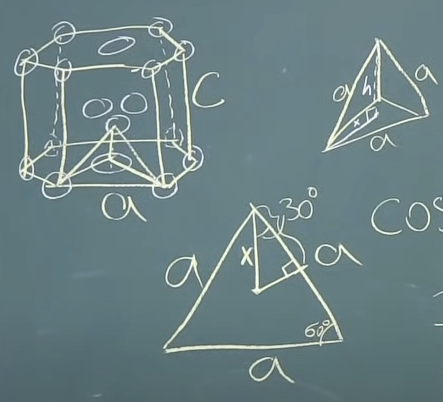
\includegraphics[width=0.5\textwidth]{hcp.png}
\end{figure}
As these diagrams show, using trigonometry we can get $\cos(30^\circ) = \frac{a}{2x}$, so $x = \frac{a}{\sqrt{3}}$. Since we know that the relation must hold with $h=\frac{c}{2}$:
\begin{equation}
    h^2+x^2 = a^2 \implies \left(\frac{c}{2}\right)^2 + \left(\frac{a}{\sqrt{3}}\right)^2 = a^2 \implies \frac{c^2}{4} + \frac{a^2}{3} = a^2 \implies \frac{c^2}{4} = \frac{2a^2}{3} \implies \left(\frac{c}{a}\right)^2 = \frac{8}{3} 
\end{equation}
And then we get the ideal ratio of $c/a = \sqrt{\frac{8}{3}} \approx 1.63$.
\subsection{Part b}
Let's start with the simple task of figuring out the density in the body-centered cubic arrangement. We know that the volume is given by $a^3$, where $a$ is the lattice constant, which in the cubic phase is 4.23 angstroms, suggesting that the volume of the unit cell is $4.23^3 = 76.2$ cubic angstroms. HCP is just a hexagonal prism with height $c$. The area of a hexagon with side $a$ is $\frac{3\sqrt{3}a^2}{2}$, so the volume of the unit cell is $\frac{3\sqrt{3}a^2c}{2}$. Since we know the ideal ratio, we can express $c=\sqrt{\frac{8}{3}}a$. The number of atoms in both the BCC and HCP unit cells is 2, so we can just compare volumes given that the density is constant during the phase transition. Equating the volumes, we get
\begin{equation}
    76.2 = \frac{3\sqrt{3}a^2\left(\sqrt{\frac{8}{3}}a\right)}{2} \implies a \approx 4.32 \text{ angstroms}
\end{equation}
\section{Problem 5}
Ashcroft and Mermin, Chapter 4, Problem 6
\subsection{Part a}
First, we want to find the packing fraction for face-centered cubic. Here, it is useful to note that the diagonal of the cubic unit cell has a value of \(a\sqrt{2}\). The volume of the unit cell is then \(a^3\), where \(a\) is the lattice constant. This diagonal accommodates 4 radii in this packing arrangement, 1 for both corners and 2 for the face centers. The volume of the spheres is then \(\frac{4}{3}\pi r^3\), where \(r = \frac{a\sqrt{2}}{4}\). Substituting gives
\begin{equation}
    \frac{4}{3}\pi r^3 = \frac{4}{3}\pi \left(\frac{a\sqrt{2}}{4}\right)^3 = \frac{4\pi \times 2\sqrt{2}a^3}{3 \times 64} = \frac{\pi\sqrt{2}a^3}{24}
\end{equation}
But each of the face-centered spheres contributes one half to the unit cell ($6 \times \frac{1}{2} = 3$ for 6 cases), and then each of the 8 corner spheres contributes \(\frac{1}{8}\) to the unit cell ($8 \times \frac{1}{8} = 1$). So we are really able to pack 4 complete spheres into the unit cell, which has the total cubic volume. The packing fraction is then
\begin{equation}
    \frac{4 \times \frac{\pi\sqrt{2}a^3}{24}}{a^3} = \frac{\pi\sqrt{2}}{6} \approx 0.74
\end{equation}
\subsection{Part b}
Next, we want to find the packing for body-centered cubic. The volume of the unit cell is \(a^3\), where \(a\) is the lattice constant. By application of the Pythagorean theorem, we find that the diagonal of the body-centered cubic is \(a\sqrt{3}\). Again this length is accommodating 4 radii, 1 for 2 corners and 2 for the body center. So the radius is \(r = \frac{a\sqrt{3}}{4}\). The volume of the spheres is then
\begin{equation}
    \frac{4}{3}\pi r^3 = \frac{4}{3}\pi \left(\frac{a\sqrt{3}}{4}\right)^3 = \frac{4\pi \times 3\sqrt{3}a^3}{3 \times 64} = \frac{\pi\sqrt{3}a^3}{16}
\end{equation}
But each of the body-centered spheres contributes unity to the unit cell ($1 \times 1 = 1$ for 1 case), and then each of the 8 corner spheres contributes \(\frac{1}{8}\) to the unit cell ($8 \times \frac{1}{8} = 1$). So we are really able to pack 2 complete spheres into the unit cell, which has the total cubic volume. The packing fraction is then
\begin{equation}
    \frac{2 \times \frac{\pi\sqrt{3}a^3}{16}}{a^3} = \frac{\pi\sqrt{3}}{8} \approx 0.68
\end{equation}
\subsection{Part c}
Next, we want to find the packing for simple cubic. The volume of the unit cell is \(a^3\), where \(a\) is the lattice constant. The lattice constant is the diameter of the sphere, so the radius is \(r = \frac{a}{2}\). The volume of the spheres is then
\begin{equation}
    \frac{4}{3}\pi r^3 = \frac{4}{3}\pi \left(\frac{a}{2}\right)^3 = \frac{\pi a^3}{2 \times 8} = \frac{\pi a^3}{6}
\end{equation}
There are 8 corners, each contributing \(\frac{1}{8}\) to the unit cell. So we are really able to pack 1 complete sphere into the unit cell, which has the total cubic volume. The packing fraction is then
\begin{equation}
    \frac{\frac{\pi a^3}{6}}{a^3} = \frac{\pi}{6} \approx 0.52
\end{equation}
\subsection{Part d}
Finally, we look at the packing for the diamond lattice. Even though it has the face-centered cubic conventional unit, the only bonds between atems occur across the body diagonal, which we know has length \(a\sqrt{3}\). The tetrahedral bond length between atoms occurs at one fourth of the body diagonal, so this suggests that the radius of the spheres is one eighth of the body diagonal, or \(r = \frac{a\sqrt{3}}{8}\). The volume of the spheres is then
\begin{equation}
    \frac{4}{3}\pi r^3 = \frac{4}{3}\pi \left(\frac{a\sqrt{3}}{8}\right)^3 = \frac{4\pi \times 3\sqrt{3}a^3}{3 \times 512} = \frac{\pi\sqrt{3}a^3}{128}
\end{equation}
But within the conventional unit cell, we see that there are 6 face-centered sites contributing $6\times\frac{1}{2} = 3$, 8 corner sites contributing $8\times\frac{1}{8} = 1$, and 4 internal sites contributing $4\times 1 = 4$. So we are really able to pack 8 complete spheres into the unit cell, which has the total cubic volume. The packing fraction is then
\begin{equation}
    \frac{8 \times \frac{\pi\sqrt{3}a^3}{128}}{a^3} = \frac{\pi\sqrt{3}}{16} \approx 0.34
\end{equation}

\section{Problem 6}
Ashcroft and Mermin, Chapter 5, Problem 1
\subsection{Part a}
As suggested, we want to prove that $b_1 \cdot\left(b_2 \times b_3\right)=\frac{(2 \pi)^3}{a_1 \cdot\left(a_2 \times a_3\right)}$. The first step will be to substitute in 
\begin{equation}
\mathbf{b}_1=2 \pi \frac{\mathbf{a}_2 \times \mathbf{a}_3}{\mathbf{a}_1 \cdot\left(\mathbf{a}_2 \times \mathbf{a}_3\right)}
\end{equation}
We have the denominator with this and we just need to prove that
\begin{equation}
    2 \pi (\mathbf{a}_2 \times \mathbf{a}_3) \cdot\left(\mathbf{b}_2 \times \mathbf{b}_3\right)=(2 \pi)^3 \implies (\mathbf{a}_2 \times \mathbf{a}_3) \cdot\left(\mathbf{b}_2 \times \mathbf{b}_3\right)=(2 \pi)^2
\end{equation}
We can use the vector triple product identity to simplify the left-hand side
\begin{equation}
    (\mathbf{a}_2 \times \mathbf{a}_3) \cdot\left(\mathbf{b}_2 \times \mathbf{b}_3\right) = (\mathbf{a}_2 \cdot \mathbf{b}_2)(\mathbf{a}_3 \cdot \mathbf{b}_3) - (\mathbf{a}_2 \cdot \mathbf{b}_3)(\mathbf{a}_3 \cdot \mathbf{b}_2)
\end{equation}
The identity only correlates reciprocal vectors with the same index, so only the first term above survives and it gives $(2\pi)^2$.
\subsection{Part b}
We want to show that relations similar to the following hold:
\begin{equation}
2 \pi \frac{b_2 \times b_3}{b_1 \cdot\left(b_2 \times b_3\right)}=a_1
\end{equation}
As instructed, we begin by substituting in for just $b_3$:
\begin{equation}
    \mathbf{b}_3=2 \pi \frac{\mathbf{a}_1 \times \mathbf{a}_2}{\mathbf{a}_3 \cdot\left(\mathbf{a}_1 \times \mathbf{a}_2\right)}
\end{equation}
which gives
\begin{equation}
    2 \pi \frac{b_2 \times b_3}{b_1 \cdot\left(b_2 \times b_3\right)}=2 \pi \frac{b_2 \times \left(2 \pi \frac{\mathbf{a}_1 \times \mathbf{a}_2}{\mathbf{a}_3 \cdot\left(\mathbf{a}_1 \times \mathbf{a}_2\right)}\right)}{b_1 \cdot\left(b_2 \times b_3\right)}
\end{equation}
We can use the vector triple product identity to simplify the numerator
\begin{equation}
    b_2 \times \left(a_1 \times a_2\right) = (b_2 \cdot a_2)a_1 - (b_2 \cdot a_1)a_2 = 2\pi a_1 - 0 = 2\pi a_1
\end{equation}
So the expression simplifies to
\begin{equation}
    a_1 = \left(2\pi \right)^3 \frac{\frac{a_1}{a_3 \cdot\left(a_1 \times a_2\right)}}{b_1 \cdot\left(b_2 \times b_3\right)}
\end{equation}
But previously we found that
\begin{equation}
    b_1 \cdot\left(b_2 \times b_3\right)=\frac{(2 \pi)^3}{a_1 \cdot\left(a_2 \times a_3\right)}
\end{equation}
and if we substitute the terms, they cancel and we are left with the identity $a_1 = a_1$.
\subsection{Part c}
We know that a Bravais lattice is defined as the parallelepiped spanned by the set of primitive vectors $\mathbf{a}_1, \mathbf{a}_2, \mathbf{a}_3$. The volume of this parallelepiped is given by the scalar triple product
\begin{equation}
    V = |\mathbf{a}_1 \cdot \left(\mathbf{a}_2 \times \mathbf{a}_3\right)|
\end{equation}
Some interpretation is in order. The cross product of two vectors gives a vector that is orthogonal to the plane spanned by the two vectors with a magnitude equal to the area of the parallelogram spanned by the two vectors. The subsequent dot product gives the projection of the area vector onto the first vector, which gives the volume of the parallelepiped spanned by the three vectors. We make sure to take the absolute value of this scalar to ensure the volume is positive.
\end{document}
